\section{Protocolo}
Toda a informação presente foi obtida da documentação do \textit{Signal} \cite{signal}.

\subsection{Primitivas}
Sem contar com os algoritmos referidos nas subsecções abaixo, que são uma grande parte do que torna o \textit{Signal} seguro, este também usa as primitivas, atualmente, mais seguras.

Algumas das primitivas e algoritmos que o \textit{Signal} utiliza são:
\begin{itemize}
    \item \textbf{\textit{SHA-512}}
    \begin{itemize}
        \item É uma função \textit{hash} criptográfica cuja operação mapeia dados de comprimento variável em dados de comprimento fixo, sendo os dados de comprimento fixo característicos do texto original e difíceis de reverter \footnote{difícil de encontrar duas mensagens com a mesma hash e difícil de  encontrar o texto original.}.
        \item Este algoritmo apresenta um número de combinações dado pela equação:
        \begin{equation}
            Combinacoes=2^{bits}=2^{512}=1.340781^{154}
        \end{equation}

        \item Isto implica que se alguém com um computador, imaginemos, a fazer $2^{16}$ cálculos em $\approx 0.2s$, isto é $327680$ cálculos por segundo, demoraria o seguinte intervalo de tempo a calcular todas essas combinações:
        \begin{equation}
            Tempo = 1.340781^{154} / 327680 = 4.091739^{148}s = 4.735809^{143} dias = 1.297482^{141} anos
        \end{equation}

        \item Colocando isto em perspetiva, sendo que a Terra tem $4,543\times10^9$ anos, um típico computador demoraria $1500 "Terras"$ a obter o total de combinações necessárias, isto é, seria necessário $1500$ vezes o tempo que a Terra existe para poder decifrar uma \textit{hash} efetuada com este algoritmo:
        \begin{equation}
        Tempo = 1.297482^{141} /4,543*10^{9} = 1.5740434^{18} ~= 1500 Terras
        \end{equation}
    \end{itemize}

    \item \textit{\textbf{Curve25519}}
    \begin{itemize}
        \item É uma curva elíptica que garante $128 bits$ de segurança, com \textit{elliptic curve Diffie-hellman key agreement}. Este foi construído de forma a evitar potenciais \textit{pitfalls} e para ser imune a \textit{time attacks} \footnote{ataques com base na análise do tempo gasto para executar algoritmos criptográficos.}.
    \end{itemize}

    \item \textit{\textbf{VXEdDSA}}
    \begin{itemize}
        \item É um algoritmo de \textit{signing} que usa a hash \textit{SHA-512}. Este funciona da seguinte forma:
        \begin{itemize}
            \item Sendo \textbf{k} uma chave privada Montgomery, \textbf{M} uma mensagem a ser assinada, \textbf{Z} uma sequência de 64 bytes aleatórios e seguros, \textbf{u} a chave publica Montgomery, \textbf{V||h||s} a assinatura a verificar(sequência de bytes em que \textbf{V} faz \textit{encode} de um ponto e \textbf{h} e \textbf{s} fazem \textit{encode} do \textit{integer modulo q(prime number)}), então temos os algoritmos dados pelo pseudocódigo em \ref{vxeddsa_sign} e \ref{vxeddsa_verify}:
            
            \begin{lstlisting}[caption=Assinatura de um documento,captionpos=b, label={vxeddsa_sign}]
                vxeddsa_sign(k, M, Z):
                    A, a = calculate_key_pair(k)
                    Bv = hash_to_point(A || M)
                    V = aBv
                    r = hash3(a || V || Z) (mod q)
                    R = rB
                    Rv = rBv
                    h = hash4(A || V || R || Rv || M) (mod q)
                    s = r + ha (mod q)
                    v = hash5(cV) (mod 2b)
                    return (V || h || s), v
                \end{lstlisting}
            
            \begin{lstlisting}[caption=Validação de assinatura de um documento,captionpos=b, label={vxeddsa_verify}]
                vxeddsa_verify(u, M, (V || h || s)):
                    if u >= p or V.y >= 2|p| or h >= 2|q| or s >= 2|q|:
                        return false
                    A = convert_mont(u)
                    Bv = hash_to_point(A || M)
                    if not on_curve(A) or not on_curve(V):
                        return false
                    if cA == I or cV == I or Bv == I:
                        return false
                    R = sB - hA
                    Rv = sBv - hV
                    hcheck = hash4(A || V || R || Rv || M) (mod q)
                    if bytes_equal(h, hcheck):
                        v = hash5(cV) (mod 2b)
                        return v
                    return false
            \end{lstlisting}
        \end{itemize}
    \end{itemize}
\end{itemize}

\subsection{KDF chains}\label{sec:KDF}
\textit{KDF Chains} faz parte do \emph{core} de um dos principais métodos, \emph{Double Ratchet} (secção \ref{sec:DoubleRatchet}), necessários para manter o \textbf{\textit{Signal}} seguro.
Este algoritmo recebe um \textbf{segredo}, uma \textbf{chave aleatória \textit{KDF}} e dados de \emph{input} e retorna um \emph{output} indistinguível de um qualquer texto gerado aleatóriamente, isto se a chave não for conhecida.
O termo \emph{KDF Chain} é usado quando parte do \emph{output} de uma \emph{KDF} é usado para substituir a \textbf{chave aleatória \textit{KDF}}, podendo assim esta ser usada para outro \emph{input}. O diagrama \ref{diagram:kdfChain} representa o processo de 3 \emph{inputs} produzirem 3 novas \emph{output keys}.


\begin{figure}[H]
\begin{center}
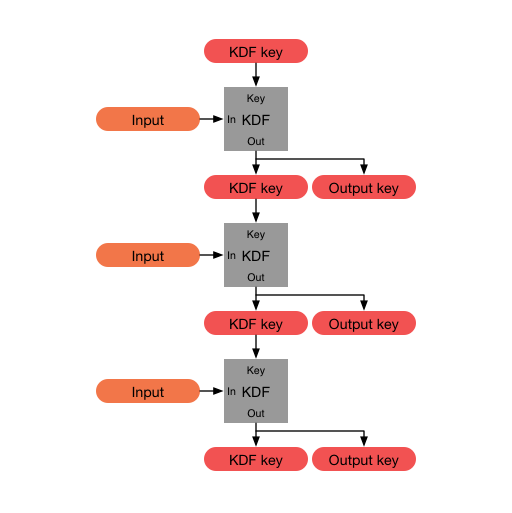
\includegraphics[width=12cm]{img/kdfChain.png}
\caption{KDF Chain com 3 inputs}
\label{diagram:kdfChain}
\centering
\end{center}
\end{figure}

Uma \emph{KDF Chain} apresenta as seguintes propriedades:

\begin{itemize}
    \item \textbf{Resiliência:} Se não houver conhecimento da chave KDF, as chaves de output aparentam ser \emph{random}. Isto mantém-se verdadeiro mesmo que o atacante controle parte dos \emph{inputs}
    \item \textbf{Forward Security:} Chaves de \textit{output} do passado aparentam ser \emph{random} para um atacante que conheceu uma chave KDF num momento futuro.
    \item \textbf{Break-in recovery:} Se os inputs futuros adicionarem entropia suficiente , as chaves \textit{output} do futuro aparentam ser \emph{random} para um atacante que conheceu uma chave KDF num momento qualquer
\end{itemize}

Numa sessão que utilize \textbf{Double Ratchet} (secção \ref{sec:DoubleRatchet}), imaginemos entre a Alice e o Bob, cada utilizador guarda 3 chaves uma para cada KDF chain: \textbf{root chain}, \textbf{sending chain},\textbf{receiving chain}. A chave \textit{sending} da Alice é equivalente à chave \textit{receiving} do Bob.

Por cada mensagem enviada e/ou recebida a \emph{chain} "avança" e as suas chaves de \emph{output} São usadas para encriptar e desencriptar as mensagens a este processo dá-se o nome de \textbf{symmetric-key ratchet}.

\subsection{Symmetric-key ratchet}\label{sec:symkey}
Todas e qualquer mensagem enviada ou recebida é encriptada usando uma \textbf{chave de mensagem única}. Esta chave única corresponde a uma chave de \textit{output} das \textit{KDF Chains} (secção \ref{sec:KDF} correspondentes. Chamemos a estas chaves \textit{chain keys}.

Os \textit{inputs} na KDF Chain para envio e receção são constantes, por esta razão não fornecem \textit{break-in recovery}. As suas chains apenas garantem que cada mensagem é encriptada com uma chave única que pode ser eliminada após encriptação ou desencriptação.Calcular a próxima chave da \textit{chain} e de mensagem corresponde a um simples \textit{ratchet step} no algoritmo \textit{symmetric-key ratchet}.
O diagrama em baixo (diagrama \ref{diagram:skRatchet} demonstra a execução deste algoritmo efetuando 2 \textit{ratchet steps}.

\begin{figure}[H]
\begin{center}
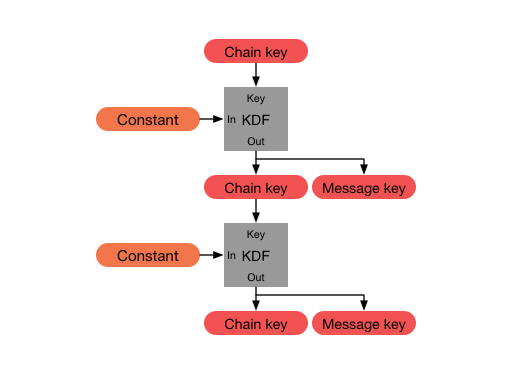
\includegraphics[width=12cm]{img/skRatchet.png}
\caption{Symmetric-key ratchet with 2 steps}
\label{diagram:skRatchet}
\centering
\end{center}
\end{figure}

\subsection{Diffie-Hellman ratchet}\label{sec:dhratchet}
Até este momento mencionamos \textit{KDF chains e Symmetric-key ratchet} ,sendo estes algoritmos necessários para o funcionamento do \textit{Double Ratchet}, no entanto estes por si só não garantem que um atacante possuindo \textit{receiving chain keys} ou \textit{sending chain keys} não consiga gerar as futuras chaves e desencriptar todas as mensagens futuras. Para evitar isto o \textbf{\textit{Signal}} combina \textit{symmetric-key ratchet} com \textit{DH Ratchet}.

Para implementar um Diffie-Hellman ratchet, cada usuário gera um par de chaves Diffie-Hellman (\textit{\textbf{ratchet key pair}}). Todas as mensagens trocadas entre estes 2 usuários vão ter no header a \textbf{chave publica}. Quando o receptor recebe a chave publica do emissor é efetuado um \textbf{DH ratchet step} que consiste em substituir o actual \textbf{\textit{ratchet key pair}} por um novo par.

Este processo leva a que ambos usuários estejam constantemente a trocar as \textbf{\textit{ratchet key pair}}, desta forma se um dos usuários for comprometido, isto é, se um atacante obter a chave privada da \textit{ratchet} apenas fica comprometida uma mensagem e todas as mensagens anteriores e posteriores continuam seguras.

Os diagramas que se seguem,juntamente com o texto que os acompanham, demonstram mais especificamente o processo do \textbf{DH Ratchet}.


A Alice é 'inicializada' com a \textit{ratchet key} publica do Bob. Desta forma a chave publica da Alice ainda não é conhecida pelo Bob. A Alice executa um calculo \textit{Diffie-Hellman} entre a sua \textit{ratchet key} private e a \textit{ratchet key} publica do Bob.

\begin{figure}[H]
\begin{center}
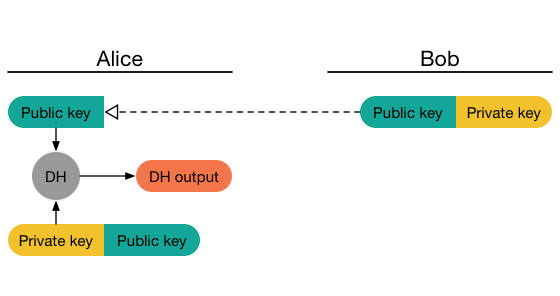
\includegraphics[width=12cm]{img/DH1.png}
\caption{Mensagem enviada do Bob para a Alice}
\label{diagram:DH1}
\centering
\end{center}
\end{figure}

A primeira mensagem enviada pela Alice anuncia a sua \textit{ratchet key} publica. Quando o Bob recebe uma destas mensagens ele calcula um \textit{DH output} entre a \textit{ratchet key} publica da Alice e a sua \textit{ratchet key} privada, o que garante (através das propriedades do \textit{DH}), caso não tenha havido um \textit{middle-man} ,que seja igual ao \textit{output} inicial da Alice. O Bob ,posteriormente, substitui o seu par de \textit{ratchet keys} e calcula um novo \textit{DH output}.

\begin{figure}[H]
\begin{center}
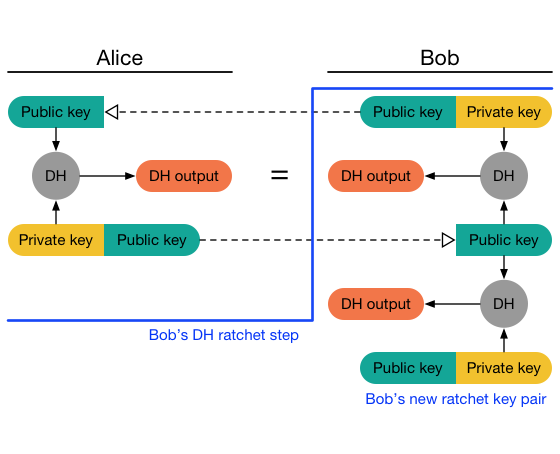
\includegraphics[width=12cm]{img/DH2.png}
\caption{Mensagem enviada da Alice para o Bob após a mensagem inicial }
\label{diagram:DH2}
\centering
\end{center}
\end{figure}

Uma nova mensagem vinda do Bob anuncia a sua nova \textit{ratchet key} publica. Quando a Alice receber esta mensagem vai executar um passo de \textit{DH ratchet}, substituindo a o seu par de \textit{ratchet keys} e derivando 2 novos \textit{DH outputs}, um que será equivalente ao ultimo \textit{DH output} do Bob e um novo para ser usado na próxima mensagem.

\begin{figure}[H]
\begin{center}
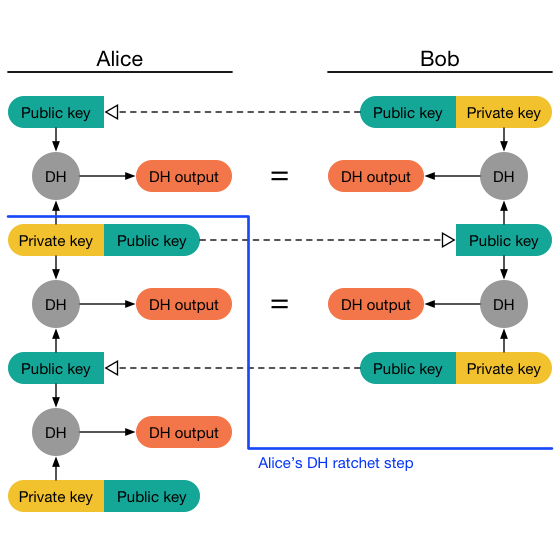
\includegraphics[width=12cm]{img/DH3.png}
\caption{Nova mensagem do Bob com a Alice como destinatário}
\label{diagram:DH3}
\centering
\end{center}
\end{figure}

Uma mensagem nova por parte da Alice anuncia a sua nova chave publica. Eventualmente o Bob ira receber uma destas mensagens e executar um passo de \textit{DH ratchet} e assim sucessivamente.

\begin{figure}[H]
\begin{center}
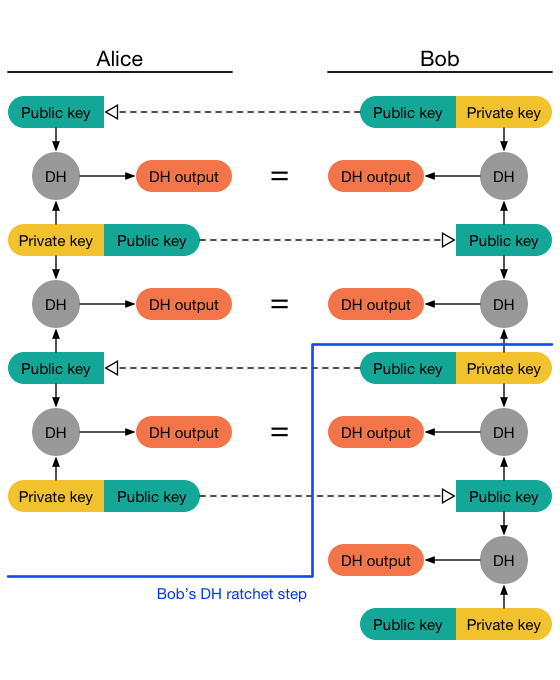
\includegraphics[width=12cm]{img/DH4.png}
\label{diagram:DH4}
\caption{Nova mensagem por parte da Alice}
\centering
\end{center}
\end{figure}

Os \textit{DH output} que são gerados em cada passo de \textit{DH ratchet} São usados para derivar novas chaves de envio e receção. A imagem em baixo revisita o primeiro passo do \textit{DH ratchet} efetuado pelo Bob. Nesta imagem o Bob usa o seu primeiro \textit{DH output} para derivar a sua chave de receção que será equivalente a chave de envio por parte da Alice.

\begin{figure}[H]
\begin{center}
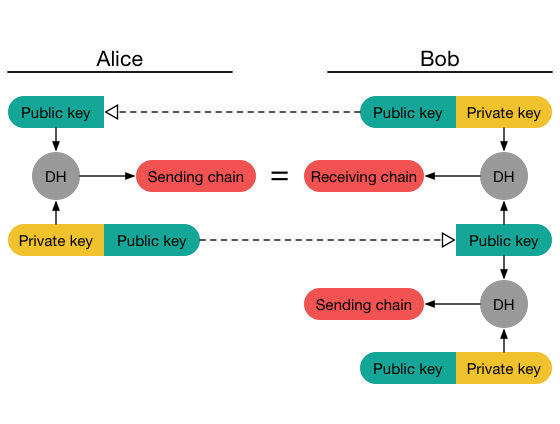
\includegraphics[width=12cm]{img/DH5.png}
\caption{Mensagem inicial por parte do Bob e resposta por parte da Alice , mostrando mais especificamente as cadeias de receção e de envio}
\label{diagram:DH5}
\centering
\end{center}
\end{figure}

Sendo que os usuários efetuam \textit{"turnos"} a executar um passo do \textit{DH Ratchet} , cada um toma turnos a introduzir novas cadeias de envio:

\begin{figure}[H]
\begin{center}
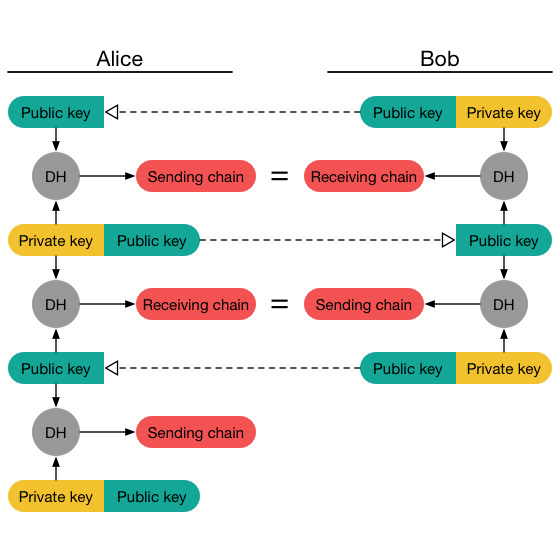
\includegraphics[width=12cm]{img/DH6.png}
\caption{Nova mensagem por parte do Bob, mostrando as cadeias de receção e de envio}
\label{diagram:DH6}
\centering
\end{center}
\end{figure}

No entanto a imagem em cima (fig. \ref{diagram:DH6}), é uma simplificado. Em vez de se usar diretamente os \textit{DH outputs}, estes são usados como \textit{KDF (\ref{sec:KDF}) inputs} para uma \textit{root chain}, sendo os \textit{KDF outputs} da \textit{root chain} usados como chaves de envio e receção. Usar \textit{KDF} aumenta a resiliência e \textit{break-in recovery}.

Desta forma ,um passo completo de uma \textit{DH Ratchet} consiste em atualizar a \textit{root KDF chain} $2\times$ e usar as \textit{DH output keys} como as novas chaves de envio e receção.

\begin{figure}[H]
\begin{center}
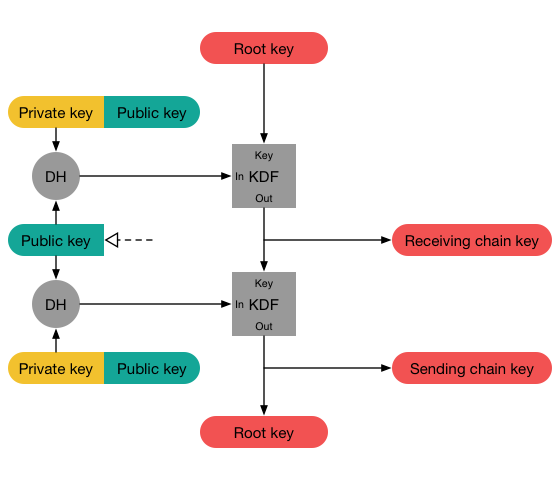
\includegraphics[width=12cm]{img/DH7.png}
\caption{Imagem que demonstra o processo por de trás da geração das cadeias mencionadas nas imagens \ref{diagram:DH5} e \ref{diagram:DH6}}
\label{diagram:DH7}
\centering
\end{center}
\end{figure}

\subsection{Double Ratchet}\label{sec:DoubleRatchet}
\subsubsection{Para que serve Double Ratchet?}
O algoritmo \emph{Double Ratchet} é um algoritmo usado por dois usuários (aplicação móvel) na troca de mensagens encriptadas baseadas numa chave secreta partilhada entre ambos. Ambos usuários derivam uma nova chave por cada mensagem de forma a que chaves anteriores não possam ser calculadas através da chaves mais recentes. Os usuários enviam valores públicos de \emph{Diffie-Hellman} juntamente com as suas mensagens. Os resultados dos cálculos de \emph{Diffie-Hellman} São misturados com a chave derivada anteriormente de modo a que chaves anteriores não possam calcular chaves mais recentes. Estas propriedades garantem proteção perante das mensagens encriptadas caso exista o comprometimento das chaves de um dos usuários.

\subsubsection{Como funciona a Double Ratchet?}
A algoritmo de \textit{\textbf{Double Ratchet}} é a combinação de \textit{Symmetric-Key (sec.\ref{sec:symkey})} com \textit{DH Ratchets (sec. \ref{sec:dhratchet})} :

\begin{itemize}
    \item Quando uma mensagem é enviada ou recebida, uma passo de \textit{Symmetric-Key ratchet} é aplicado nas cadeias de envio ou receção para derivar a nossa chave da mensagem.
    \item Quando uma nova chave \textit{ratchet public} é recebida, um passo de \textit{DH ratchet} é efetuado antes da \textit{symmetric-key ratchet} para substituir as chaves da cadeia ( \textit{chain keys})
\end{itemize}

No diagrama \ref{diagram:DR1} ,em baixo, a Alice inicializou o processo com a chave \textit{ratchet public} e um segredo partilhado (equivalente à chave raiz inicial). Na inicialização a Alice gera um novo par de chaves \textit{ratchet} e envia o \textit{DH output} para a raiz do \textit{KDF} de forma a que sejam calculadas uma nova chave raiz e uma nova chave de envio.

\begin{figure}[H]
\begin{center}
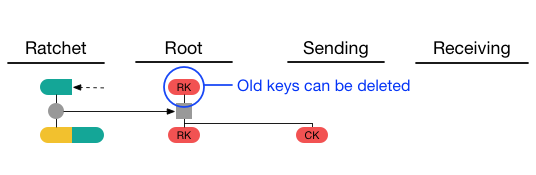
\includegraphics[width=12cm]{img/DR1.png}
\caption{Primeira mensagem por parte do Bob e inicialização da chave raiz e chave de envio}
\label{diagram:DR1}
\centering
\end{center}
\end{figure}

Quando a Alice envia a sua primeira mensagem, ela aplica um passo \textit{symmetric-key ratchet} à sua cadeia de chaves de envio, resultando numa nova chave para mensagens ( cada chave deste género possuirá um \textit{label} perante a mensagem que estas encriptam/ desencriptam). A nova chave da cadeia é guardada enquanto a chave para mensagem e a antiga chave de cadeia podem ser eliminadas.

\begin{figure}[H]
\begin{center}
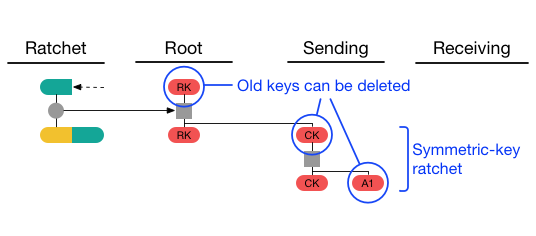
\includegraphics[width=12cm]{img/DR2.png}
\caption{Demonstração de um passo na symmetric-key ratchet após receção da primeira mensagem}
\label{diagram:DR2} 
\centering
\end{center}
\end{figure}

Se posteriormente a Alice receber uma mensagem vinda do Bob, esta irá conter uma nova chave \textit{ratchet public}. A Alice aplica um passo de \textit{DH ratchet} de forma a derivar novas chaves de envio e receção. Posteriormente aplica um passo \textit{symmetric-key ratchet} na cadeia de receção para obter a chave de receção para a mensagem vinda do Bob.

\begin{figure}[H]
\begin{center}
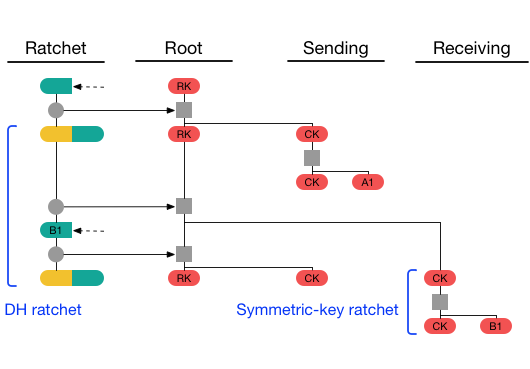
\includegraphics[width=12cm]{img/DR3.png}
\caption{Demonstração de um passo na symmetric-key ratchet após receção da segunda mensagem vinda do Bob levando à geração de uma chave de receção}
\label{diagram:DR3} 
\centering
\end{center}
\end{figure}

Suponhamos que a Alice envia uma mensagem A2, recebe uma mensagem B2 ( com a chave \textit{ratchet public} antiga ), depois envia a mensagem A3 e A4. A cadeia de envio da Alice faz 3 passos enquanto a sua cadeia de receção apenas andou 1 passo.

\begin{figure}[H]
\begin{center}
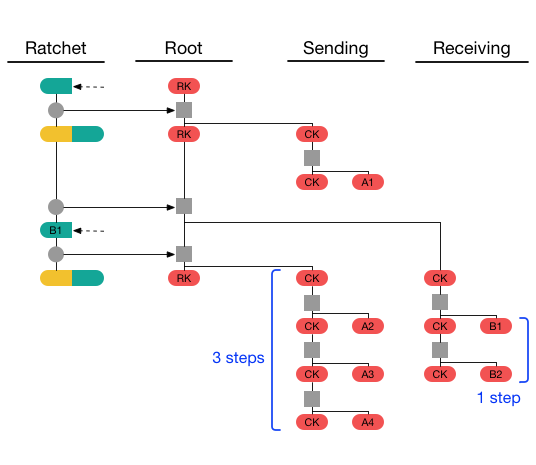
\includegraphics[width=12cm]{img/DR4.png}
\caption{Demonstração de alguns casos específicos do Double-Ratchet}
\label{diagram:DR4} 
\centering
\end{center}
\end{figure}

Se ,posteriormente, receber a mensagem B3 e B4 com a próxima chave \textit{ratchet} do Bob e em seguida enviar a mensagem A5 o seu estado final será como identificado no diagrama \ref{diagram:DR5}.

\begin{figure}[H]
\begin{center}
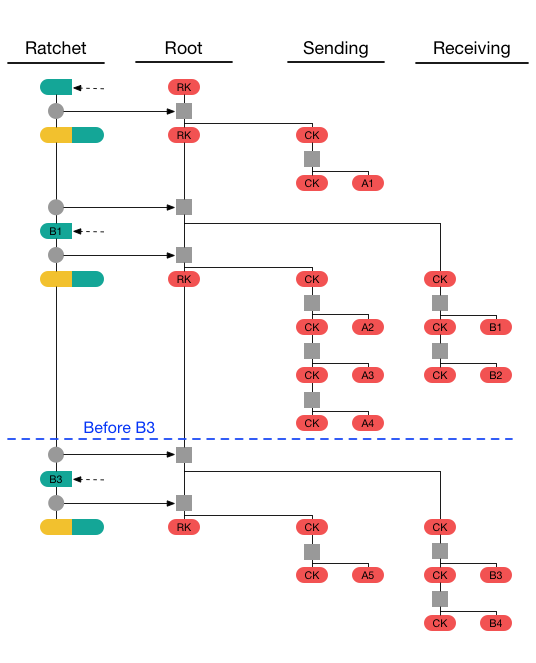
\includegraphics[width=12cm]{img/DR5.png}
\caption{Estado final da cadeia}
\label{diagram:DR5} 
\centering
\end{center}
\end{figure}

\subsection{Será o protocolo do \textit{Signal} realmente seguro?}
Perante tudo o que foi mencionado nos protocolos usados pelo \textit{Signal}, rapidamente poderíamos considerar que sim, o \textit{Signal} seria um protocolo bastante seguro. No entanto, sem qualquer acesso ao \textit{source-code}, não conseguimos validar realmente o quão solido e seguro é o \textit{Signal}. Aqui entra uma das grandes razões para o \textit{Signal} ser o protocolo e aplicação mais segura de todas as existentes (sendo até usado por entidades políticas de grandes países \cite{politicsSignal}), pois o \textit{Signal} é \textbf{\textit{Open-Source}}, permitindo que qualquer pessoa veja o código e detete erros no mesmo, o que até aos dias de hoje ainda não aconteceu. O protocolo utilizado pelo \textit{Signal} foi tão popular,seguro e tão bem recebido que ficou a ser um protocolo por si mesmo tendo sido este adaptado em 2018 por grandes empresas como \textbf{WhatsApp},\textbf{Facebook Messenger},\textbf{Skype} e \textbf{Google Allo}, apesar disso em alguns destes o protocolo \textit{Signal} não se encontra ativado por defeito.

Excluindo o que foi mencionado em cima, o \textit{Signal} ainda proporciona uma excelente documentação \cite{signal} onde explica detalhadamente todo o processo por detrás do seu protocolo o que permite que qualquer engenheiro valide o protocolo sem olhar para o código , podendo detetar lacunas antes de olhar para o \textit{source-code}.
Por outro lado o \textit{Signal} tem passado por varias auditorias sem qualquer registo de falhas a nível de segurança.

Algumas auditorias e estudos feitos ao \textit{Signal}:
\begin{itemize}
    \item 2014,Outubro, investigadores de \textit{Ruhr University Bochum} publicam uma análise do protocolo \textbf{validando a sua segurança} \cite{frosch2016secure}.
    \item 2016,Outubro, investigadores de \textit{University of Oxford,Queensland University of Technology and McMaster University} publicam uma analise formal do protocolo concluído que o protocolo era \textbf{criptograficamente seguro} \cite{cohn2017formal}.
    \item 2017,Julho, investigadores de \textit{Ruhr University Bochum} durante uma nova análise detetam uma falha puramente teórica, uma vez que esta ao acontecer seria automaticamente detetada, voltando a \textbf{validar a declaração anterior} \cite{rosler2018more}.
\end{itemize}

\subsection{O que torna o protocolo do \textit{Signal} superior?}
Tendo sido adaptado pelas grandes empresas, como mencionado em cima, não se consideraria um protocolo pouco robusto mas ,para realçar uma das suas grandes vantagens é o facto de ser \textbf{\textit{Open-Source}} o que permite que uma grande comunidade de pessoas com gosto por \textit{\textbf{infosec}} possam ver o \textit{source-code} e detetar falhas sem ser por tentativa e erro através de uma interface (como mencionado anteriormente). Enquanto o \textit{Signal} é \textit{Open-Source} e sabemos que a comunicação é realmente \textbf{\textit{end-to-end encrypted}} , e se duvidarmos podemos facilmente ver o \textit{source-code} e confirmar. 

As outras ferramentas estão fechadas ao publico e não permitem acesso ao código desta forma, apenas podemos confiar que as entidades se estão a comportar e não estão a fazer nada de errado com os nossos dados. Em cima disto como falado em cima o \textit{Signal} tem sofrido bastantes auditorias e estas não encontraram qualquer problema com a aplicação.

Ao contrario do \textit{WhatApp}, o \textit{Signal} não guarda dados (ou metadados que por vezes ainda são mais importantes) do cliente e se este quiser privacidade o \textit{Signal} garante-a enquanto o \textit{WhatsApp}, sendo a aplicação mais utilizada , não o faz o que põe em causa a privacidade de milhões de usuários. O \textit{WhatsApp} apesar de usar o protocolo seguro e open-source do \textit{Signal} pode ,\textit{behind the curtains}, estar a fazer algo mais que desconhecemos.O \textit{WhatsApp} efetua um \textit{load} de todos os nossos contactos do telemóvel para os seus servers remotos de forma a detetar quem tem ou não WhatsApp enquanto o \textit{Signal} usa a tecnologia \textit{\textbf{SGX}} da Intel (regiões protegidas da memória). 

Comparativamente ao \textit{Telegram} ,para além da distinção que o \textit{Telegram} não é \textit{open-source} e o \textit{Signal} é , o \textit{Signal} perante as analises feitas possui um algoritmo de segurança muito superior ao do Telegram.
O \textit{Signal} apaga \textbf{completamente},ênfase no completamente, as mensagens passado algum tempo, enquanto noutras apps, \textit{Telegram} inclusive, os records mantém-se guardados num servidor caso sejam apagadas.

Além de tudo o referido anteriormente o \textit{Signal} encontra-se ativamente a procurar manter a privacidade dos seus clientes mesmo que sejam impostas regras pelos países onde estes vivem.

\subsection{Domain Fronting e \textit{Signal} App}
Em grande parte a sociedade procura ter privacidade ,no entanto, no outro lado existem organizações ,muitas vezes políticas, que pretendem obter mais informação sobre a população ou dos cidadãos do seu pais. Desta forma , alguns países como por exemplo o Egito (e.g Egito bloqueia todas as comunicações \textit{Signal} \cite{noSignal}), bloqueiam o tráfego de aplicações como o \textit{Signal} , consequentemente reduzindo a privacidade das pessoas.

O \textit{Signal} entrevem neste aspeto, mais uma vez procurando devolver a privacidade aos cidadãos, usando um mecanismo chamado \textbf{\textit{Domain Fronting}}. Este mecanismo ,como referido no artigo \cite{domainFrontingExplained}, funciona fazendo \textit{bypass} aos métodos de censura que bloqueiam através de \textit{DPI,DNS Filtering e IP Blocking} , sendo que estes dependem de grandes \textit{CDN's}. Desta forma o \textit{Domain Fronting} não passa de uma maneira de fazer o tráfico parecer que é gerado por um \textit{domain} válido, isto apenas é possível pela forma como as \textit{CDN's} modernas funcionam, tudo isto acontece na \textit{application layer da camada OSI (figura \ref{diagram:OSI})}. 
Por exemplo, o \textbf{Domain A} e o \textbf{Domain B} pertencem ao mesmo \textit{CDN}, no entanto o \textbf{A} encontra-se bloqueado mas o \textbf{B} não. Assim a ideia principal do \textit{Domain Fronting} é criar um pacote com o \textbf{Domain B} no \textit{SNI Header} e o \textbf{Domain A} no \textit{HTTP Header}. Uma vez que o \textit{SNI} não é encriptado no \textit{TLS Protocol} este não sera bloqueado pelas autoridades, mas quando o pedido chega ao CDN e lê o HTTP Host Header com o \textit{Domain A} este será encaminha para o \textit{Domain A}(fig. \ref{diagram:domainFronting}).

Como podemos ver o \textit{Signal} tenta sempre possibilitar e manter a privacidade dos seus usuários ,no entanto este método deixa de funcionar se ,como mencionado no artigo do \textit{Signal} \cite{signalDomainFronting},se bloquearem todos os sites de um \textit{CDN} especifico para se bloquear o site que se pretende censurar (e.g Tentativa da Russia a bloquear o \textit{Telegram} bloqueiam todo o tráfego de uma \textit{CDN} \cite{domainFrontingBlock} \cite{domainFrontingExplained} ). No final de contas o \textit{Signal} perdeu ,nos países em que foi censurado, pois as \textit{CDN's} bloquearam este tipo de comportamento (e.g Amazon Services bloqueia \textit{Signal} \cite{signalDomainFronting}), mas deixou uma marca que demonstra que ,internamente,o seu protocolo visa e procura manter a privacidade das pessoas.

\begin{figure}[H]
\begin{center}
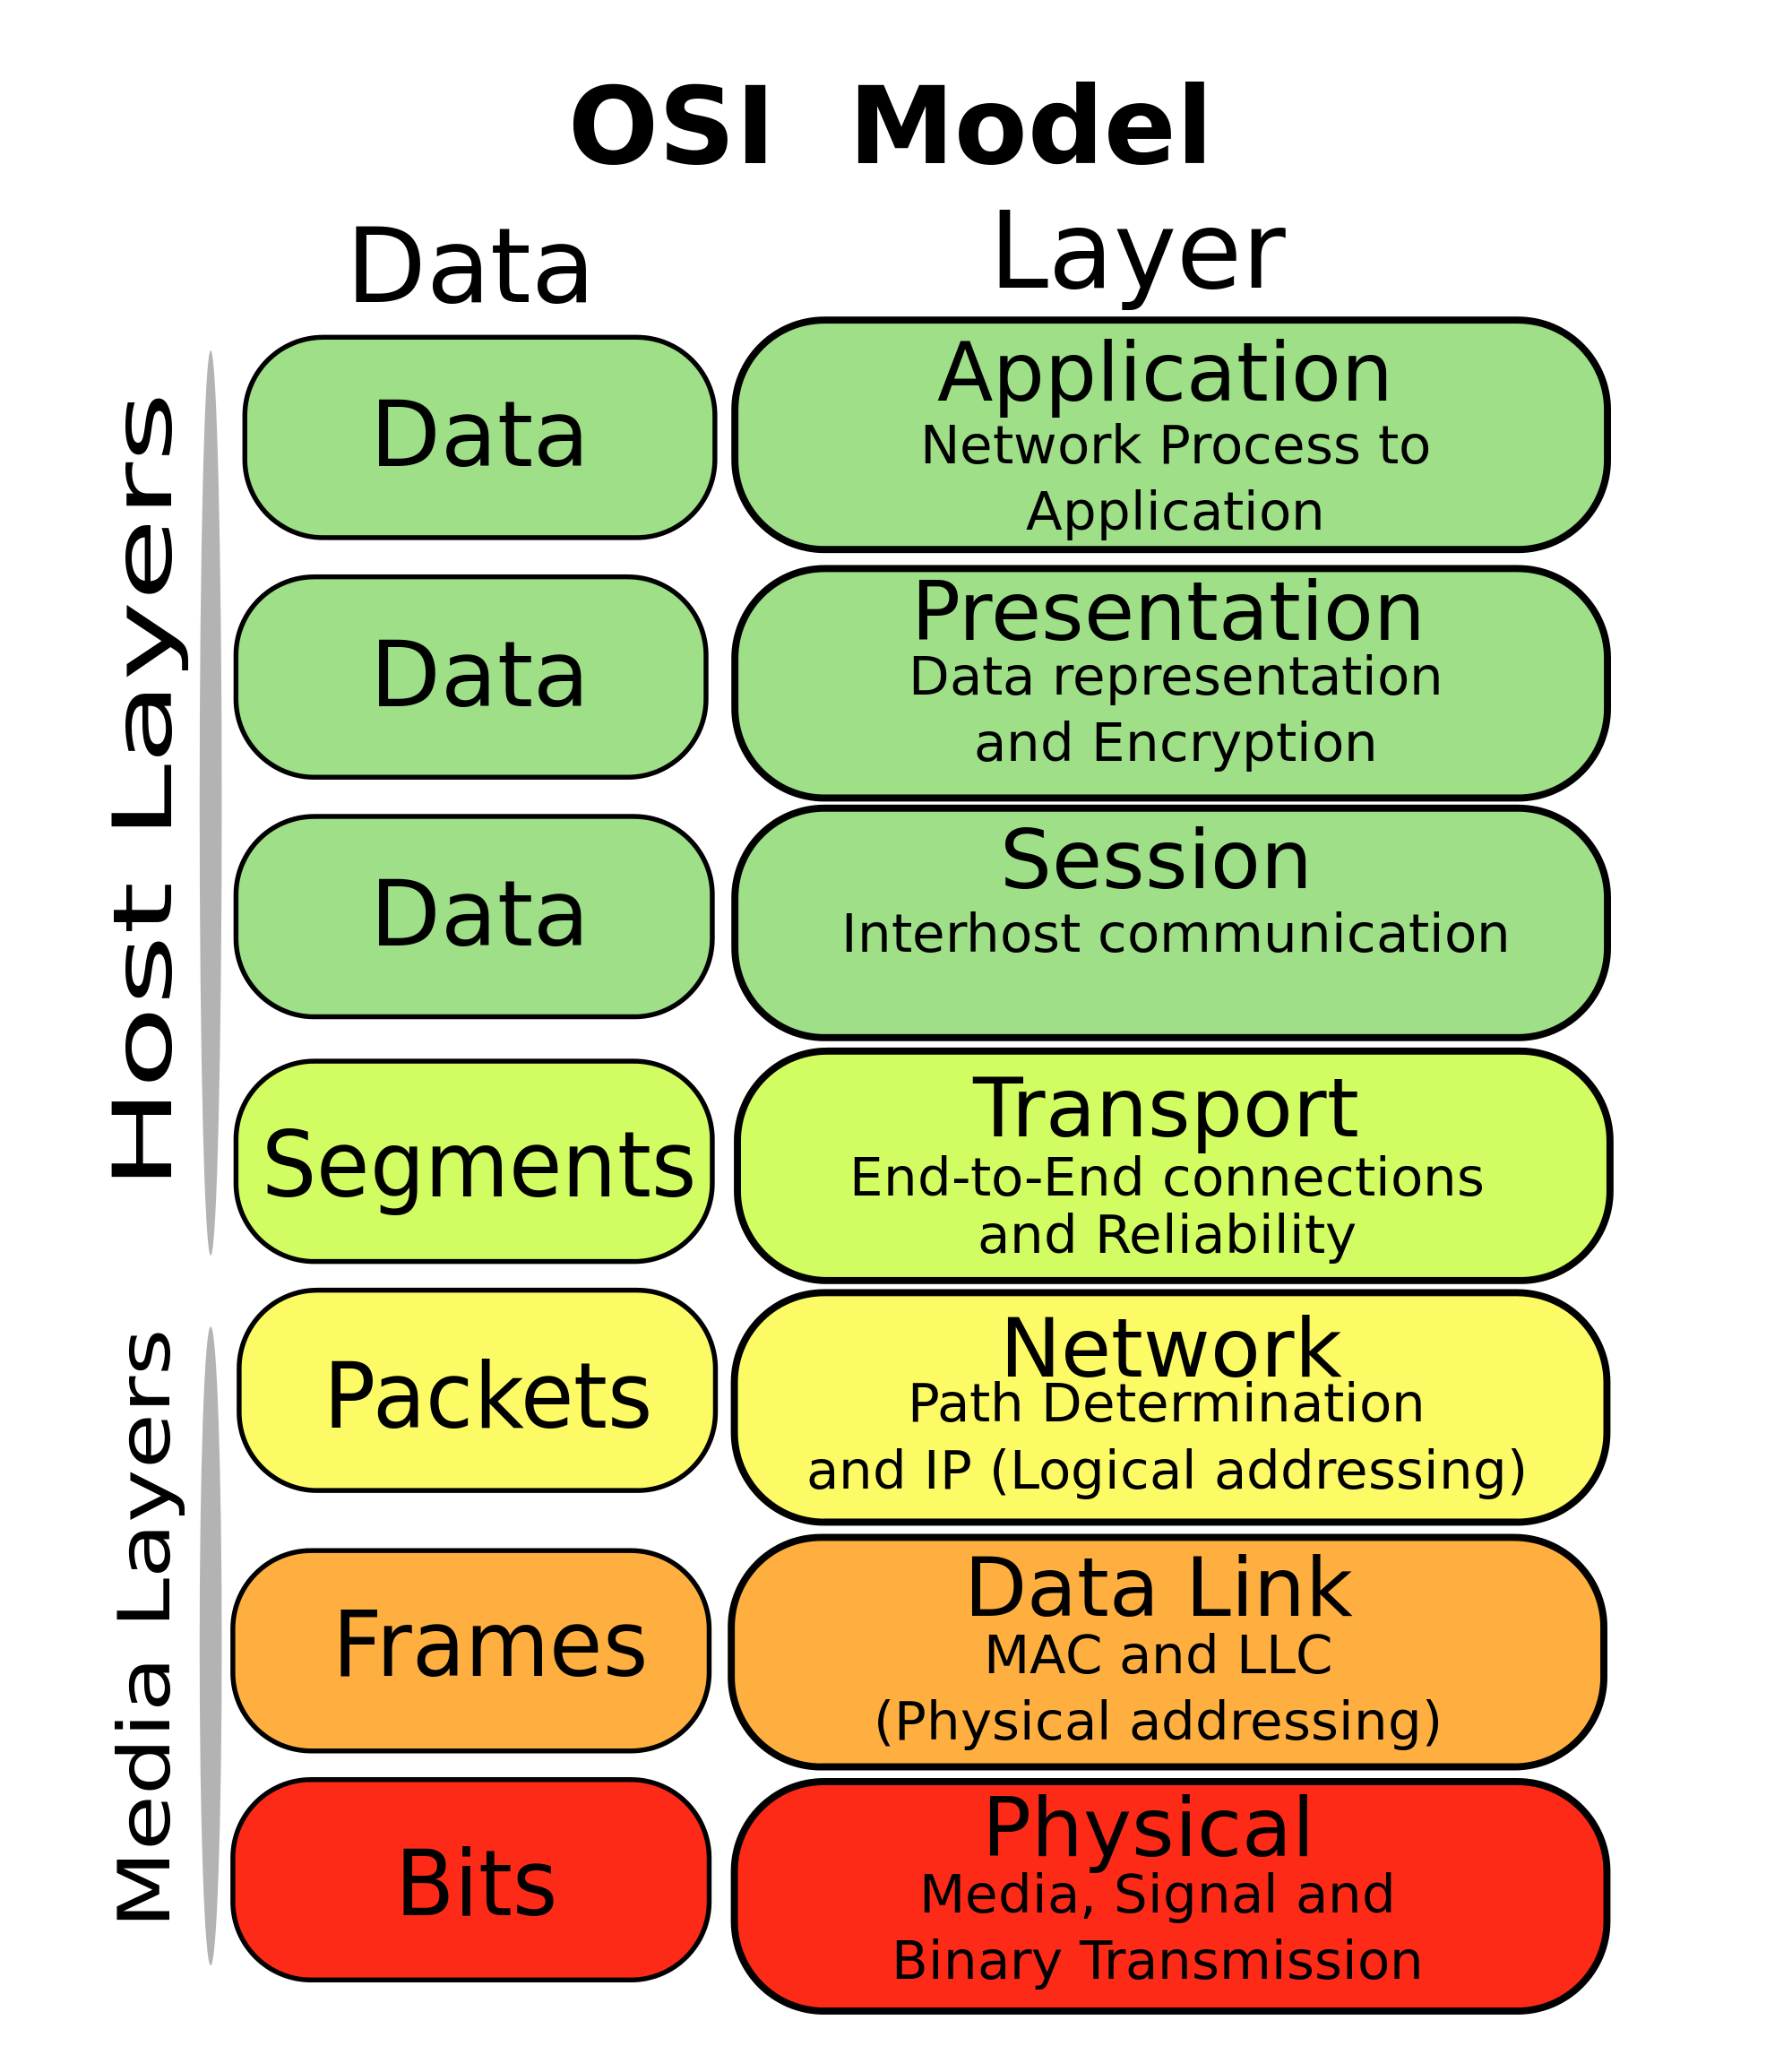
\includegraphics[width=12cm,height=10cm]{img/OSI.png}
\caption{Figura representativa das camadas OSI, dando ênfase à camada aplicacional \cite{OSI}.}
\label{diagram:OSI}
\centering
\end{center}
\end{figure}

\begin{figure}[H]
\begin{center}
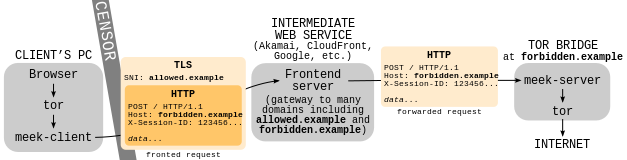
\includegraphics[width=15cm]{img/domainFronting.png}
\caption{Funcionamento do Domain Fronting \cite{df}.}
\label{diagram:domainFronting}
\centering
\end{center}
\end{figure}
